\documentclass{article}
\usepackage[utf8]{inputenc}
\usepackage{graphicx}
\usepackage{amsthm}
\newtheorem{problem}{Problem}
\newtheorem{extension}{Extension}


\title{AMPD}
\author{Josh's Problems}
\begin{document}

\maketitle

\begin{problem}
Grendel the witch is cooking up a storm! She is brewing potions in several cauldrons.

Grendel needs to make at least three potions at a time, so she need to use at least 3 cauldrons at once. If the cauldrons have a radius of 3 feet and Grendel must be equally close to all cauldrons used what is the shortest distance Grendel can be from the center of a cauldron?

There is a special right triangle which might help you on your answer. The 30, 60, 90 triangle! Let x be the side opposite of the $60^o$ angle. Let y be the side opposite the $90^o$ angle. It must be that $y = \frac{2}{\sqrt{3}}x$.

\begin{figure}[h!]
\centering
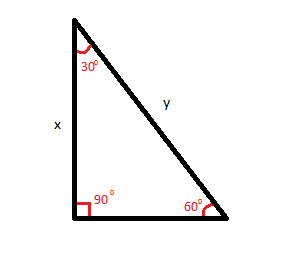
\includegraphics[scale=.5]{triangle}
\end{figure}

\end{problem}

\begin{proof}
Since Grendel is equally close to the center of every cauldron used, these centers lay on a big circle with Grendel as the center. The distance to Grendel is minimized by making no gaps between any two cauldrons. As we use fewer and fewer cauldrons the radius of this “big circle” is minimized. This means using 3 cauldrons minimizes the distance from Grendel to a cauldron.


\begin{figure}[h!]
\centering
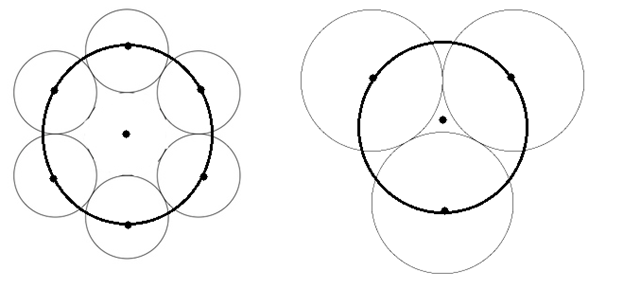
\includegraphics[scale=.5]{circles}
\end{figure}

To determine how close Grendel is in the circle to the right we note the triangle formed by connecting the three circle centers and note Grendel is equally close to them.

\begin{figure}[h!]
\centering
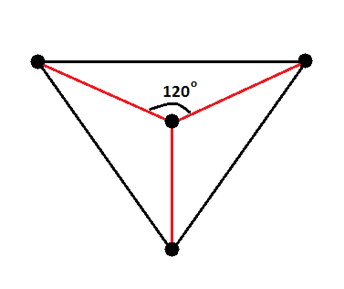
\includegraphics[scale=.5]{bigtri}
\end{figure}

The black lines are equal length and the red lines are equal length so we have 3 equivalent isosceles triangles within an equilateral triangle. So the three angles at the center all equal to one another and sum up to $360^o$. This means each of these angles is $120^o$.

Now let's look at just the "top two" circle centers, as well as Grendel.

\begin{figure}[h!]
\centering
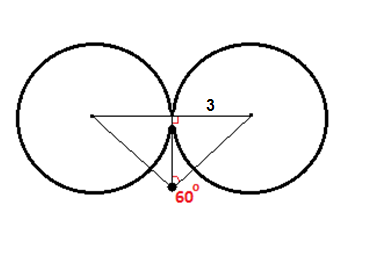
\includegraphics[scale=.5]{circletri}
\end{figure}

By drawing upward from Grendel we will cut the segment between the two circle centers in half. However, what we've really done is form a 30, 60, 90 triangle whose side opposite to the $60^o$ angle is 3. The hypotenuse of this triangle happens to be the distance we are trying to find so all we must do now is use the formula we were given at the start: $y = \frac{2}{\sqrt{3}}x$. (Where y is the hypotenuse and x is the side opposite to the $60^o$ angle)

Plugging is 3 for x yields $y= \frac{6}{\sqrt{3}}=2\sqrt{3}$.
\end{proof}

\begin{extension}
Grendel decided she's working too hard so she got her brooms to do the work for her. Grendel set up several brooms and cauldrons in her basement. Every broom is equally close to 3 cauldrons and is $\frac{2}{\sqrt{3}}$ feet away from them. What is the maximum number of brooms a single cauldron can be $\frac{2}{\sqrt{3}}$ feet away from? What shape do all the brooms surrounding one cauldron form?
\end{extension}
\begin{proof}
6, a hexagon.
\end{proof}

\begin{problem}
Count Calcula is making plans to build a new part of Transylvania. The cost to construct a building is 100 dragon teeth per road leading to that building. He wants you to determine the cost of the three plans below.
\\
\\
Plan A)

\begin{figure}[h!]
\centering
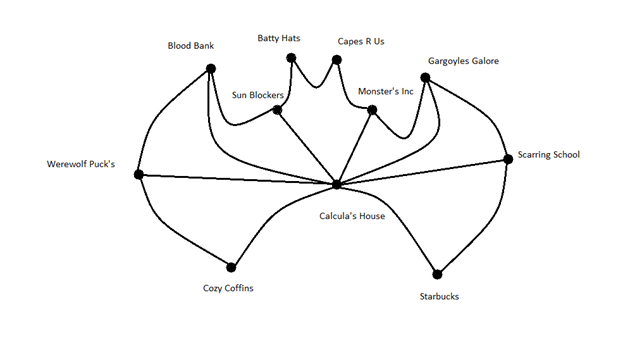
\includegraphics[scale=.7]{plana}
\end{figure}



Plan B)
\begin{figure}[h!]
\centering
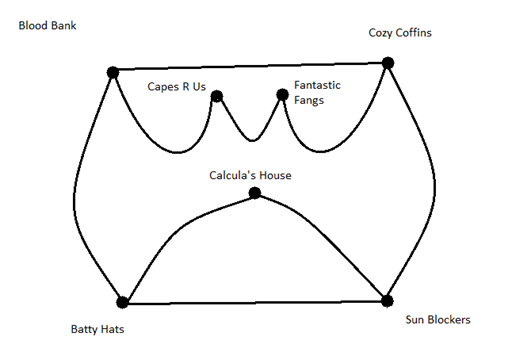
\includegraphics[scale=.7]{planb}
\end{figure}
\\
\\
Plan C)
Igor misplaced the blueprints to Plan C but says there are 75 roads.
\end{problem}
\begin{proof}
This problem is essentially the degree-sum formula for graph theory. The degree of a building is the number of roads which lead to it. Adding up the degrees of every building will actually count the number of road twice. Why? Every road leads to exactly two buildings, meaning every road contributes exactly 2 to the sum of degrees.

With this in mind we see Plan A has 17 roads, so the sum of degrees of every building is 34 meaning it will cost 3400 dragon teeth to construct Plan A.

Plan B has 9 roads, so 18 is the sum of degrees meaning it will cost 1800 dragon teeth.

Plan C has 75 roads, so 150 is the degree-sum meaning it will cost 15,000 dragon teeth.
\end{proof}

\begin{extension}
A ghost city will be built around the new addition to Transylvania and follows a few rules which make haunting easier. The rules are as follows:

1) Every space in Transylvania must have exactly one ghost building.

2) A ghost road is made if it joins two ghost buildings by crossing over a road in Transylvania.


Below is the ghost city of Transylvania Plan B:
\begin{figure}[h!]
\centering
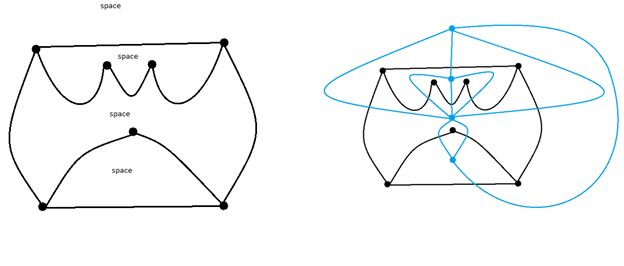
\includegraphics[scale=.7]{ghostplans}
\end{figure}

If Transylvania Plan D has 33 roads what is the cost of constructing the ghost city?

If the length of a space is the number of roads the space touches what is the sum of lengths of spaces in Plan D?
\end{extension}
\begin{proof}
Cost: 6600 dragon teeth. Length-sum: 66
\end{proof}

\end{document}
